\documentclass{article}
\usepackage[T1]{fontenc} %Better support for european accented chars
\usepackage[utf8]{inputenc} %Enables danish chars and other good stuff
\usepackage{lmodern} 
\usepackage{amssymb}
\usepackage{csquotes} % qoute in danish
\usepackage[danish]{babel}
\usepackage{pstricks-add}
\usepackage{lastpage} %Package for getting the number of the last page.
\usepackage{graphicx} %Allows insertion of graphics
\usepackage{amsmath} %Gives better math support.
\usepackage{amsfonts} %Gives additional fonts.
\usepackage{amssymb} %Adds additional symbols.

%Pakker der bruges for at lave klikbare links i pdf filer
\usepackage{varioref} %Gives the \vref{lbl} command that make nice references that includes page numbers.
\usepackage[pdftex, colorlinks=false, pdfauthor={\authorText}, pdftitle={\titleText}]{hyperref} %Makes references clickables in the pdf file. colorlinks can be set to true for colored links.
\usepackage{memhfixc} %Solves problems with hyperref in Memoir, to be loaded after hyperref.

\usepackage{url}
\usepackage{pdfpages}
\usepackage{listings}
\usepackage{color}
\usepackage{todonotes}
\usepackage{url} % Nice url look
\usepackage[backend=bibtex,style=alphabetic]{biblatex} %Bibliography package.
%\usepackage{anysize}
%\marginsize{3cm}{3cm}{1.5cm}{4cm} % venstre, højre, top, bund.
\lstset{literate=%
{æ}{{\ae}}1
{å}{{\aa}}1
{ø}{{\o}}1
{Æ}{{\AE}}1
{Å}{{\AA}}1
{Ø}{{\O}}1
}

\definecolor{mygreen}{rgb}{0,0.6,0}
\definecolor{mygray}{rgb}{0.5,0.5,0.5}
\definecolor{mymauve}{rgb}{0.5,0,0.3}
\definecolor{myblue}{rgb}{0,0.4,0.9}
\pagestyle{plain}

\bibliography{19_del3} %Choose the bibliography to load, file to be called name.bib.

\begin{document}
\section*{Projektopgave efterår 2013 - jan 2014}
\section*{02312-14 Indledende programmering og 02313 Udviklingsmetoder til IT-Systemer}
Projektnavn: \textcolor{red}{del3}
Gruppe nr: \textcolor{red}{19}
Afleveringsfrist: \textcolor{red}{mandag den 02/12 2013 Kl. 5:00}
\\\\
Denne rapport er afleveret via Campusnet (der skrives ikke under)
\\\\
Denne rapport indeholder \textcolor{red}{77} sider incl. denne side
\\\\
Studie nr, Efternavn, Fornavne
\\\\
\textcolor{red}{s110795, Mortensen, Thomas Martin}
\\
Kontakt person (Projektleder)
\\\\
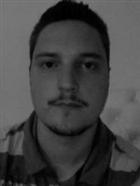
\includegraphics[scale=0.5]{ThomasM.jpg}
\\\\
\textcolor{red}{s113577, Johansen, Chris Dons}
\\\\
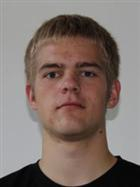
\includegraphics[scale=0.5]{ChrisJ.jpg}
\\\\
\textcolor{red}{s123897, Ahlgreen, Thomas Kamper}
\\\\
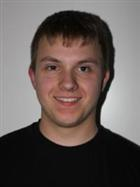
\includegraphics[scale=0.5]{ThomasA.jpg}
\newpage
\section*{Timeregnskab}
\begin{tabular}{|c|c|c|c|c|c|c|r|} \hline
 Dato & Deltager & Design & Implementering & Test & Dok. & Andet & I alt \\ \hline
&&&&&&& \\ \hline
 15/11-13 & Thomas Mortensen & 2& & & & & 2\\ \hline
 15/11-13 & Chris Johansen & 2& & & & &2 \\ \hline
 15/11-13 & Thomas Ahlgreen & 2& & & & & 2\\ \hline
 &&&&&&& \\ \hline
 22/11-13 & Thomas Mortensen & & 2,5& & & &2,5 \\ \hline
 22/11-13 & Chris Johansen & &2,5 & & & &2,5 \\ \hline
 22/11-13 & Thomas Ahlgren & & 2,5& & & &2,5 \\ \hline
 &&&&&&& \\ \hline
 29/11-13 & Thomas Mortensen & &2,5 & & & &2,5 \\ \hline
 29/11-13 & Chris Johansen & &2,5 & & & & 2,5 \\ \hline
 29/11-13 & Thomas Ahlgren & &2,5 & & & & 2,5 \\ \hline
 &&&&&&& \\ \hline
 2/12-13 & Thomas Mortensen & & &1 &6 & &7 \\ \hline
 2/12-13 & Chris Johansen & & &1 &6 & &7 \\ \hline
 2/12-13 & Thomas Ahlgren & & &1 &6 & &7 \\ \hline
 &&&&&&& \\ \hline
 diverse & Thomas Mortensen & & & &4 & & \\ \hline
 diverse & Chris Johansen & & & & &2 & \\ \hline
 diverse & Thomas Ahlgren & & & & & & \\ \hline
 &&&&&&& 48\\ \hline
\end{tabular}
\newpage
\tableofcontents
\newpage
\section{Indledning}
Spilfirmaet IOOuterActive har givet os endnu en opgave.

Kundens vision er en udvidelse af vores allerede udviklede programmer fra \cite{19del1} og \cite{19del2}

Denne gang ønsker kunden at lave flere forskellige typer felter. Disse felter skal implementeres på en "rigtig" spilleplade, hvor man kan gå i ring. Samtidig ønskes der mulighed for 2-6 spillere. Spillerens konto skal sættes med et fast beløb fra start, og spillet skal slutte, når en spiller er gået bankerot.


Projektet forventes at have elementer fra både \textbf{FURPS+} og \textbf{GRASP}. Herudover er der lavet specifikke krav til hvilke artefakter, der skal ingå i krav, analyse, kode, test, og designdokumentation.
\\

OBS: alle gruppemedlemmer er lige ansvarlige for alle dele af vores dokumentation
\section{Kravspecificering og Use cases}
I dette afsnit vil vi beskrive vores kravspecificering og vores Use cases, som vi har udarbejdet til denne rapport.
\subsection{Kravspecificering}
\todo[inline]{Thomas M: Indsætte de få tvivlskrav, der er i dropbox}
I dette afsnit har vi taget udgangspunkt i kundens vision. Vi har læst den igennen, og stillet spørgsmålstegn, ved de ting, der kunne være tvivl om. Kunden er dog blevet til kravspecificering i forløbet, og derfor var der få tvivlsspørgsmål.
\begin{enumerate}
\item Hvad skal der ske, hvis en spiller ikke kan betale det han skal?
\item Skal man betale, hvis man lander på et felt, der er ejet af en bankerot spiller?
\item Skal man have mulighed for at købe eet felt, der tidliger var ejet af en spiller, der nu er gået bankerot?
\end{enumerate}
Vores kontakt i firmaet, som er vores projektleder, har besvaret disse punkter på følgende måde
\begin{enumerate}
\item Spilleren der ikke kan betale, må betale det han har, og går herefter bankerot.
\item Feltet er ikke længere ejet af nogen, og derfor skal der heller ikke betales.
\item Da feltet ikke længere ejes, skal man kunne købe det.
\end{enumerate}
\subsection{Use Cases}
\todo[inline]{Thomas A: Indsæt tekst fra fully dresses og brief + diagram}
Vi vil i dette afsnit beskæftige os med 2 use cases, som er beskrevet i nedenstående diagram. Til vores spil har vi lavet en fully dressed use case, og til vores test har vi blot lavet en brief use case.
\subsubsection{Use Case Diagram}
\begin{figure}[ht]
\centering
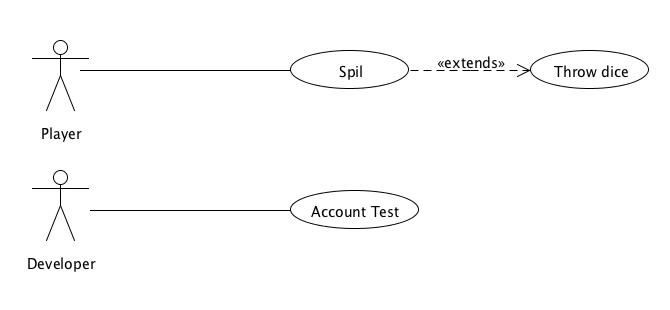
\includegraphics[scale=0.5]{UseCaseDiagram.jpg}
\caption[<Text for the list of figures>]{Use Case Diagram}
\label{fig:figure 2}
\end{figure}
\newpage
\subsubsection{Fully Dressed Use Case}
Vi har i dette afsnit beskrevet vores use case med en fully dressed use case for spil.
\subsubsection*{Use Case}
Spil
\subsubsection*{Scope}
Terningspil
\subsubsection*{Level}
User Goal
\subsubsection*{Primary actor}
Spiller
\subsubsection*{Stakeholders and Interests}
Spiller: vil vinde spillet
\subsubsection*{Preconditions}
Eclipse er installeret på maskinen.
\\
Programmet er startet.
\subsubsection*{Main Success Scenarie:}
\begin{enumerate}
\item Spiller starter spillet
\item Spiller indtaster Navn
\item Spiller Ruller med terningerne
\item Spiller lander på et felt med positiv konsekvens
\item Spiller modtager point
-- Spiller gentager punkt 3-5 indtil 3000 eller mere er opnået
\item System checker vinder
\item System viser vinder
\item System lukker ned
\end{enumerate}
\subsubsection*{Extensions Alternative scenarier:}
*a - til hvert et tidspunkt
\begin{enumerate}
\item Spiller lukker spillet ved at taste "q"
\end{enumerate}
4a. Spiller lander på et felt med negativ konsvens
\begin{enumerate}
\item Spiller får trukket point
\item Spiller ryger under 0 point
-- punkt 6-8 i main success aktiveres
\end{enumerate}
4b. Spiller lander på et felt uden konsekvens
\begin{enumerate}
\item Spiller for trukket point
\item a Spiller ryger under 0 point
-- punkt 6-8 i main success aktiveres
\item b Spiller rammer felt 10. uden at komme under 0, hviket giver ekstra tur. 
-- punkt 3 i main success aktiveres
\end{enumerate}
\subsubsection*{Specielle Krav:}
\begin{itemize}
\item Skal kunne køre på en Windows maskine med Java EE på DTU's computere
\item Skal kunne spilles af en almindelig bruger
\end{itemize}
\subsubsection{Brief Use Case Account test}
Vi har valgt at lave en brief use case over vores test.
\\

\textbf{Account Test}
En udvikler tester klassen med forskellige grænse og middelværdier, der er foruddefineret i klassen. Resultaterne printes ud i konsollen, og udvikleren ser om resultaterne fra testen, stemmer overens med de forventede resultater.
\section{FURPS+}
\todo[inline]{Thomas M: forklar furps, og hvordan vi har brugt det.}
I \textbf{UP} bruger man \textbf{FURPS+}, der er udviklet af Hewlett-Packard til at kategoriserer kravene til ens system. "\textbf{+}" i \textbf{FURPS+} kom til senere, efter HP ønskede at dække flere kategorier med denne model.
\subsection{Functional}
- Hvilke funktioner skal systemt have. Hvad skal det kunne. Sikkerhed.
\subsubsection{Hvordan har vi brugt det?}
Vi har gennem vores kravspecificering fundet ud af at systemet skulle indeholde...
\subsection{Usability}

\subsubsection{Hvordan har vi brugt det?}
\subsection{Reliability}
\subsubsection{Hvordan har vi brugt det?}
\subsection{Performance}
\subsubsection{Hvordan har vi brugt det?}
\subsection{Supportability}
\subsubsection{Hvordan har vi brugt det?}
\subsubsection*{Her kommer de underfaktorer, som +'et repræsenterer}
\subsection{Implementation}
\subsubsection{Hvordan har vi brugt det?}
\subsection{Interface}
\subsubsection{Hvordan har vi brugt det?}
\subsection{Operations}
\subsubsection{Hvordan har vi brugt det?}
\subsection{Packaging}
\subsubsection{Hvordan har vi brugt det?}
\subsection{Legal}
\subsubsection{Hvordan har vi brugt det?}
\section{Domænemodel}
\begin{figure}[ht]
\centering
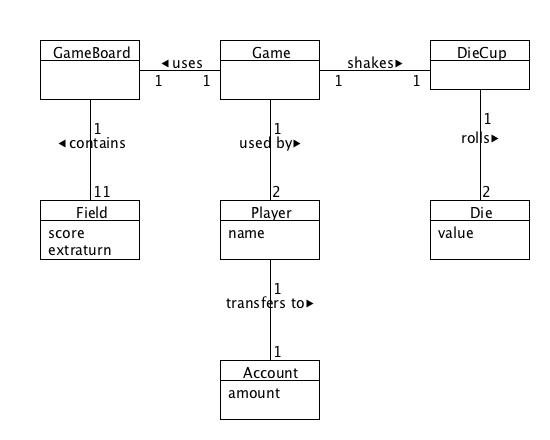
\includegraphics[scale=0.5]{DomainModelDieGame.jpg}
\caption[<Text for the list of figures>]{Domain Model}
\label{fig:figure 2}
\end{figure}
Da vi har kunnet bruge en stor del af vores domænemodel fra sidst, har vi valgt ikke at lave en navneordsanalyse, da vi ville bruge for lang tid på at lave den, i forhold til udbyttet af denne. Dette er årsagen til, at vi starter med domænemodellen.
\\

Vores domæne model er lavet før begyndelse af implementering. Det er udført forinden for at få et overblik over hvilke elementer, vi kunne have behov for i vores program. 
\\


Vi har i diagrammet vist vores hoved domæner. \textit{Game}, som er selve spillet. \textit{Gameboard}, der holder styr på indholdet i spillet. \textit{Field}, som indeholder en score for feltet, og om det giver ekstra tur. \textit{Player}, der bruger spillet. \textit{Account} holder styr på point. \textit{DieCup}, som skal rulle vores terninger. Til sidst har vi \textit{Die} som indeholder terningeværdier, vi skal bruge til at udregne, hvor spilleren lander.
\section{BCE model}
\todo[inline]{Thomas M: indsæt model og forklar}
\begin{figure}[ht]
\centering
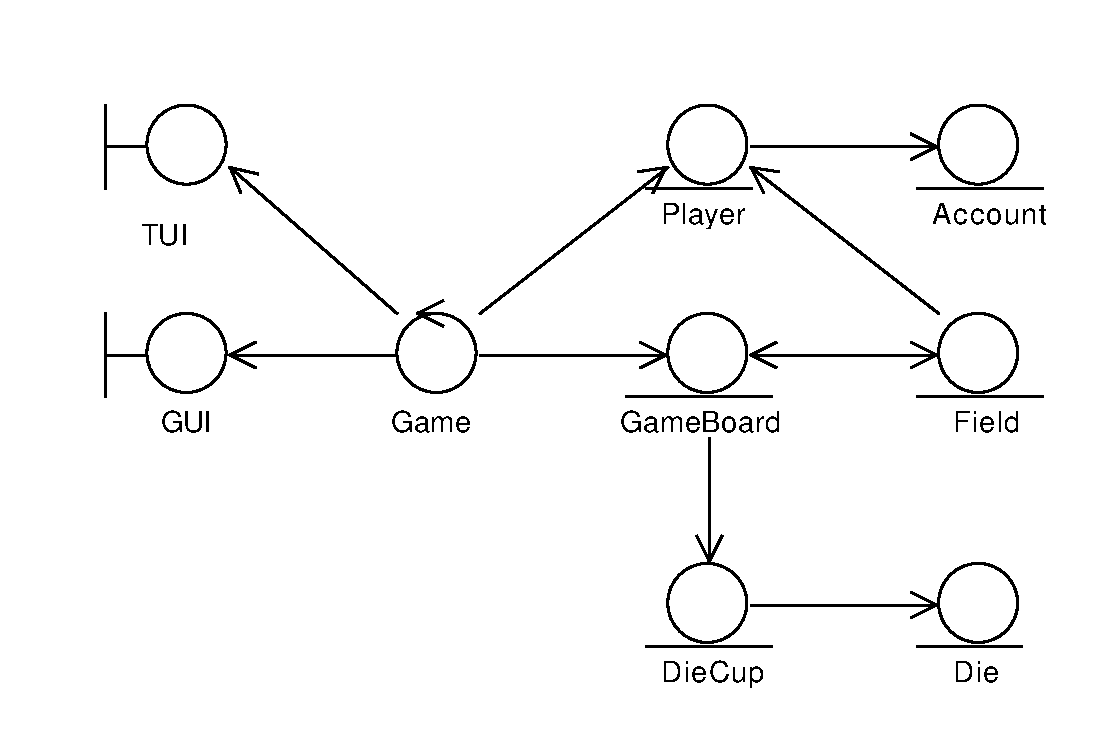
\includegraphics[width=1\textwidth]{BCEModel.pdf}
\caption[<Text for the list of figures>]{BCE Model}
\label{fig:bcemodel}
\end{figure}
I denne CDIO opgave, har vi igen benyttet os af en BCE model til at skabe oveblik over vores kendskab i koden.
\\
Vi har denne gang ændret 
\\
Det vil sige at vi i denne model kun har tilføjet vores nye entitetsklasser. Det handler om entiteterne \textit{Account}, \textit{Field}, og \textit{GameBoard}. Vi har også lavet en ny boundary vi kalder \textit{Graphic}, som bearbejder beskeder til vores importerede \textit{GUI}.
\\
Som det fremgår af diagrammet, styrer controlleren \textit{Game} stadig spillet. Det vil sige at vores controller tildeler ansvaret ud til de nære klasser.
\\
\textit{Account} er en pengebeholdning der styres af \textit{Player} klassen. Vores controller har derfor kun brug for direkte kendskab til \textit{Player}.
\\\\
\textit{Field} holder styr på felterne i spillet, og vores \textit{Gameboard} holder styr på felterne. Vores \textit{Game} controller har dermed kendskab til felterne i spillet gennem vores \textit{Gameboard}.
\\


Ud fra disse informationer kan controlleren så sende besked til vores boundary's \textit{TUI} og \textit{Graphic}, som viser brugeren konsekvenserne i spillet grafisk og i tekst. Dette er hvad \vref{fig:bcemodel} beskriver
\section{Systemsekvens Diagram}
\todo[inline]{Thomas A}
\begin{figure}[!ht]
\centering
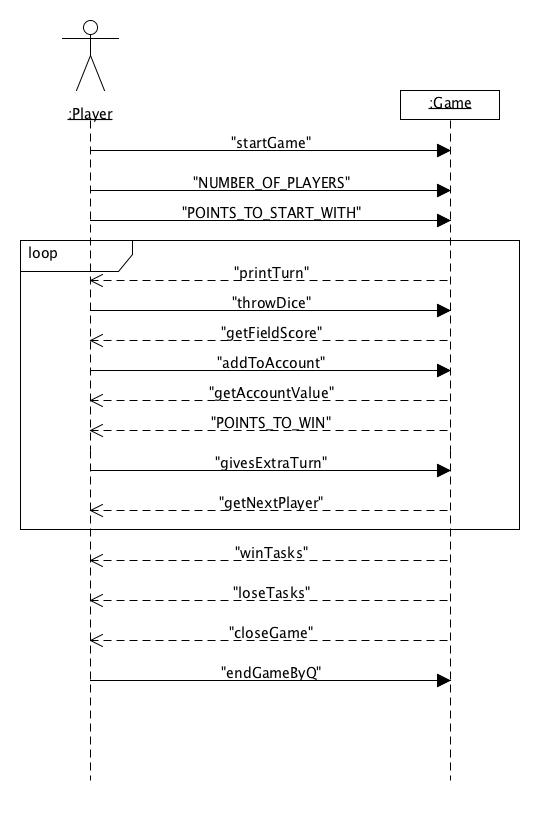
\includegraphics[scale=0.4]{SystemSequenceDiagramDieGame.jpg}
\caption[<Text for the list of figures>]{Systemsekvens Diagram}
\label{fig:figure 2} 
\end{figure}
Vores System sekvens diagram tager udgangspunkt i vores fully dressed use case: spil. Det første der sker, er at selve spillet startes. Herefter finder vi ud af hvor mange spillere, der er. Spillernes startbalance bliver nu sat. Herefter vil spillet kører i en løkke, indtil en af spillerne har tabt eller vundet. Løkken printer turen på spilleren. Terningen kastes. Spilleren får konsekvensen af det felt han lander på. Beløbet bliver overført til spillerens konto. Spilleren får nu vist hvad balancen er på kontoen. Der bliver kontrolleret, hvor vidt spilleren har opnået point nok til at vinde eller har mistet alle sine penge (Her mangler en metode til at kontrollere balancen på spillerens konto). Hvis det er tilfældet hopper vi ud af løkken. Hvis det er et bestemt felt på pladen, skal spillet give spilleren en ekstratur (Pilen vender den forkerte vej i diagrammet). Dette vil give ham en tur mere i løkken. Hvis ingen af disse ting forekommer, giver spillet turen videre. Hvis en spiller har vundet, skriver konsollen, hvilken spiller det er og hans point. Hvis en spiller har tabt, skriver konsollen, hvilken spiller der så har vundet og hans point. Efter det lukker spillet. Spilleren har hele tiden mulighed for at stoppe spillet med tasten "q".
\\
Systemsekvensdiagrammet er vigtigt at have med, da det vise hvordan systemet reagere på udefrakommende inputs. Det giver også indblik i hvordan systemet skal fungere uden at skulle skrive en masse kode.
\section{Kode}
Her vil vi forklare hvordan vi har grebet selve koden an.
\subsection{Struktur og pakker}
Ligesom i de to foregående projekter, er programmet skrevet med fokus på at overholde \textbf{BCE}-modellen. Kort fortalt betyder det for opdelingen i pakker, at alle klasser er inddelt i pakker efter deres type ift. \textbf{BCE}. For en mere uddybende beskrivelse henvises til det tilsvarende afsnit i \cite{19del1} og \cite{19del2} rapporterne.
\subsection{Genanvendelse af kode og opbygning}
På baggrund af hensigtsmæssigt og godt design i \cite{19del1} og \cite{19del2} projekterne, har det været muligt at genbruge store dele af koden. Således er klasserne \texttt{Die} og \texttt{DieCup} i praksis identiske med de tilsvarende klasser fra de tidligere projekter, ligesom den generelle opbygning af systemet også ligner meget.

På samme måde er det grundlæggende princip bag \texttt{TUI} og \texttt{Graphic} klasserne også identisk med 19del2 – klasserne har ikke behov for at bære data, og de forskellige metoder i klasserne interagerer ikke med hinanden gennem felter eller lign, og kan derfor med fordel være statiske. For en mere dybdegående forklaring henvises til kodeafsnittet i 19del2.

\subsection{Bemærkelsesværdige løsninger}
Systemet er på nuværende tidspunkt så omfattende, at det ikke giver mening at gennemgå alle overvejelser bag implementeringen af alle klasser. I stedet uddrages specielt bemærkelsesværdige dele af koden, og forklares herunder, for at give en bedre forståelse af systemets virkemåde, uden at gennemgå alt. Beskrivelserne er opdelt efter hvilke klasser de er implementeret i.
\subsubsection{TUI}
Noget af det første der sker, når dette spil startes, er at brugeren anmodes om at indtaste antallet af spillere. Antallet af spillere må ifølge opgavebeskrivelsen ikke være større end 6, og spillet giver ikke meget mening, hvis det er mindre end 2. Med andre ord skal der specifikt indtastes et tal mellem 2 og 6. Dette er en ny udfordring ift. de tidligere opgaver, hvor der blot blev gemt en hel streng. Foruden at teste, at det indtastede tal er i det krævede interval, ønskede vi også at lave systemet robust, og sikre at f.eks. bogstaver eller specialtegn indtastet på dette tidspunkt, ikke kunne få systemet til at gå ned. Dette ses i figur \vref{fig:kode1}.
\begin{figure}[!ht]
\centering
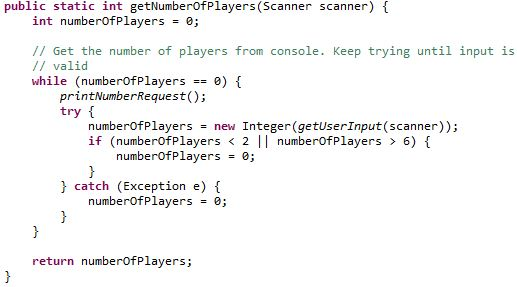
\includegraphics[width=0.8\textwidth]{kode1.jpg}
\caption[<Text for the list of figures>]{Antal spillere}
\label{fig:kode1} 
\end{figure}
Tjekket og sikringen mod karakterer som ikke er tal, sker i \texttt{TUI}, inden det sendes videre til controlleren. Antallet af spillere sættes indledningsvist til 0, og forespørgslen kører så i en løkke, som kun brydes når antallet af spillere bliver sat til noget der er forskelligt fra 0. Det input der hentes fra konsollen er som udgangspunkt en streng, og skal derfor konverteres før det kan bruges som en talværdi. Denne konvertering vil kaste en Exception, hvis der gives et input, der ikke umiddelbart giver mening som tal-værdi – f.eks. et bogstav. Det smarte er så, at denne Exception kan fanges, og kode kan udføres til at ”reparere” den fejl, som har forårsaget den. I vores tilfælde sætter vi bare værdien for antal af spillere tilbage til 0, fordi det betyder at løkken kører igen, så brugeren bliver spurgt efter et nyt input.
Ligeledes hvis der gives et input, som succesfuldt kan konverteres til en talværdi, tjekkes der om tallet er mellem 2 og 6 – hvis ikke det er det, sættes værdien tilbage til 0, og løkken kører igen. Så snart løkken brydes, returnerer metoden.

\subsubsection{GameBoard}
Ligesom ved et fysisk spil, indeholder dette system en spilleplade \texttt{GameBoard}, som er bygget op af felter af forskellig type. Disse felter er bygget i et system med arv, som beskrevet senere i dette afsnit, og dette giver en stor fordel for datastrukturen i \texttt{GameBoard}. Fordi alle de forskellige felttyper \texttt{Territory, LaborCamp, Fleet, Tax og Refuge} nedarver fra Field, kan der laves en enkelt liste (array) af felter, af typen \texttt{Field}, som kan indeholde alle de forskellige felter, selvom der er tale om forskellige typer objekter, med forskellige implementeringer af metoder mm. Koden ses i figur \vref{fig:kode2}.
\begin{figure}[!ht]
\centering
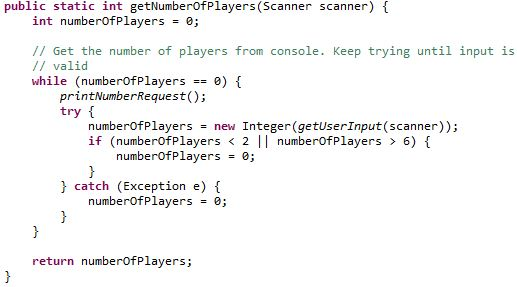
\includegraphics[width=0.8\textwidth]{kode1.jpg}
\caption[<Text for the list of figures>]{Antal spillere}
\label{fig:kode2} 
\end{figure}
\subsubsection{Field} 
Som nævnt tidligere, er felterne bygget op med at system af arv. Alle felterne nedarver fra \texttt{Field}, som indeholder de ting der er fælles for alle felter. I realiteten er det ikke ret meget der er det samme for alle felter – der er forskellige muligheder ift. køb, der er forskellige konsekvenser (få penge, miste penge), og selv de felter der har den samme konsekvens – at man skal betale til andre – har forskellige måde at beregne beløbet på.

Alle felter har dog et navn, og alle felter har mulighed for at man kan lande på dem. Derfor indeholder \texttt{Field} et felt til navn, og en abstrakt metode – \texttt{landOnField} – der betyder at alle klasser som arver fra \texttt{Field}, skal ”love” at de implementerer \texttt{landOnField}. De forskellige underklasser kan så have forskellige implementeringer af \texttt{landOnField}, så længe typen af parametre og returværdi er de samme.


To typer felter – \texttt{Tax} og \texttt{Refuge} – nedarver direkte fra \texttt{Field}, men de resterende 3 felttyper nedarver i stedet fra \texttt{Ownable}, som så igen nedarver fra \texttt{Field}. Dette skyldes, at disse 3 felter – \texttt{Territory, LaborCamp} og \texttt{Fleet} – kan købes. Dette er en funktionalitet, som grundlæggende vil virke ens for alle tre typer felter – der skal være et pegepind til en ejer, der skal være en måde at købe feltet osv.
Desuden vil den grundlæggende procedure, når der landes på feltet, også være ens – der skal tjekkes om der er nogen der ejer feltet, og hvis der er, skal der betales leje til ejeren. Hvordan lejen udregnes, er forskellige for de forskellige typer at felter, men den overordnede procedure er ens. Derfor er \texttt{landOnField}-metoden, der som bekendt skal implementeres, når klasserne arver fra \texttt{Field}, implementeret i \texttt{Ownable}. Metoden i \texttt{Ownable} kalder så \texttt{getRent-metoden}, der har forskellig implementering i hver af underklasserne.
\subsubsection{Fleet}
Af de underklasser, hvor der skal udregnes leje, er \texttt{Fleet} en af de mere interessante. Lejen for \texttt{Fleet} afhænger nemlig af hvor mange andre \texttt{Fleet}-felter ejeren af det felt der landes på, har. Det betyder, at det \texttt{Fleet}-felt der er landet på, er nødt til at kende ejeren af de øvrige \texttt{Fleet}-felter, for at kunne udregne lejen.
I praksis implementeres det ved, at et \texttt{Fleet} felt-objekt tager den spilleplade \texttt{GameBoard} det oprettes i, med som parameter, når det oprettes. Således har \texttt{Fleet}-feltet mulighed for at gå ud og se på andre felter på den samme spilleplade.

Dernæst er problematikken blot, at de objekter på spillepladen, som dette objekt nu har adgang til, er af typen \texttt{Field}. Overklassen \texttt{Field} indeholder ikke en ejer, så før ejeren af feltet kan findes, må det konverteres til \texttt{Ownable}. Herefter er det blot en simpel løkke, som tjekker ejeren på hvert \texttt{Fleet}-felt, og summerer op. Når antallet af \texttt{Fleet}s er fundet, kan lejen simpelt findes med en switch-sætning.
\subsubsection{LaborCamp}
På samme måde som \texttt{Fleet}, bruges antallet af ejede felter af samme type også til beregningen af lejen ved \texttt{LaborCamp}. Fremgangsmåden til at finde antallet af ejede felter, er helt den samme som ved \texttt{Fleet}.
Foruden antallet af ejede \texttt{LaborCamps}, indgår også et terningslag i beregningen af lejen – det betyder at \texttt{LaborCamp} er nødt til at have kendskab til \texttt{DieCup}, for at kunne få værdien af et terningslag. Imidlertid befinder\texttt{DieCup} sig på spillepladen \texttt{GameBoard}, så i kraft af at \texttt{LaborCamp} allerede har \texttt{GameBoard} med som argument, for at kunne kigge på andre felter, har den også let adgang til \texttt{DieCup}.
\subsubsection{Ownable}
Som nævnt tidligere i afsnittet, er der 3 felttyper som kan købes. Nå en spiller køber et felt, skal der trækkes nogle penge fra spillerens konto, og \texttt{owner}-pegepinden i feltet skal sættes til at pege på spillerens objekt. Før dette sker, skal der imidlertid have været præsenteret et valg for spilleren, om hvorvidt denne ønsker at købe feltet eller ej, og lige netop dette viser sig at være den mest krævende del at implementere af denne funktionalitet.


Ideen med hele opbygningen af systemet efter \textbf{BCE}-modellen er nemlig, at elementer fra entitets-laget aldrig har direkte adgang til elementer fra brugergrænseflade-laget. Men for at kunne præsentere valget om køb for spilleren, er feltet nødt til at kalde \texttt{TUI}’en, for at printe på skærmen og tage input fra konsollen – og vil netop give det føromtalte uønskede kendskab fra brugergrænsefladen til en entitet. Alternativt kunne man måske forstille sig, at feltet så havde kendskab til controlleren, og så kunne kalde TUI’en den vej igennem, men det vil også bryde mønsteret – ideen er jo at det er controlleren der skal kontrollere programmet, og kalde metoder i entiteter og brugergrænsefladen.


Uanset hvordan det drejes, er der ikke rigtigt en perfekt løsning på denne problemstilling – i hvert fald ikke uden at der skal ændres på de metoder, som er givet i opgavebeskrivelsen, der som udgangspunkt ikke må ændres. Med andre ord handler det nok om at finde den mindst dårlige løsning.


I vores projekt vælger vi at udnytte, at både felterne og controlleren har kendskab til spillerens objekt. I stedet for at kalde en metode, når en bruger lande på et felt der kan købes, sættes således et ”flag” i spillerens objekt \texttt{isOnBuyableField = true}. Når der så returneres til controlleren, kan der tjekkes på om spilleren står på et felt der kan købes, og selve købet foretages i controlleren, som jo har kendskab til både \texttt{TUI} og felterne.
\subsubsection{Tax}
Der er to typer af \texttt{Tax} – den simple, hvor der blot betales et fast beløb, og den mere avancerede, hvor der kan vælges mellem et fast beløb og en procentdel af spillerens formue. Sidstnævnte er interessant, dels fordi den er nødt til at kende ejeren af alle andre felter, for at kunne beregne spillerens formue, dels fordi den skal spørge spilleren hvilken mulighed der foretrækkes.

At beregne formuen er i store træk implementeret på samme måde som \texttt{Fleet} og \texttt{LaborCamp} – feltet tager \texttt{GameBoard} med som parameter, og kan så få fat i ejeren af de andre felter. Her summers så ikke op på antal, men på pris.


At spørge brugeren, giver til gengæld samme problematik som omtalt ved køb af felter i \texttt{Ownable} – en entitet er nødt til at ”snakke” med brugergrænsefladen. Det kunne løses på samme måde som ved køb af felter, ved at bruge spillerens objekt til at gemme et ”flag”, men forskellen er, at både det faste \texttt{Tax}-beløb og det udregnede procentvise \texttt{Tax}-beløb er nødt til at med ud til controlleren, for at der kan opkræves korrekt. Det betyder dels, at der, foruden ”flaget”, også skal gemmes to talværdier i spillerens objekt, og dels at man effektivt vil have flyttet hele logikken fra Tax ud i controlleren.
I praksis vil den løsning ganske vist løse opgaven og give pæne diagrammer, hvor der ikke er nogen synlig kobling mellem \texttt{Tax} og \texttt{TUI} – men reelt giver det en skjult kobling, som måske i virkeligheden er højere end den ville være, hvis \texttt{Tax} bare havde kendskab direkte til \texttt{TUI}, og som under alle omstændigheder er langt sværere at gennemskue.


Derfor vælger vi at lade \texttt{Tax} have kendskab til \texttt{TUI}, men knytter hertil samtidigt en klar bemærkning om, at dette er et af de steder hvor systemet kan forbedres.
\subsubsection{Game}
Strukturen og ideen i \texttt{Game}-controlleren er stadig helt den samme som i de tidligere projekter. En af de største forskelle i controlleren, er muligheden for mere end 2 spillere, og måske endnu vigtigere, det faktum at der ikke bare er en spiller som vinder – der er spillere som taber løbende, og som så skal udgå af spillet. Det betyder nemlig, at der ikke blot kan laves en simpel valgsætning, som afgør om en spiller har vundet – i stedet må der tælles hvor mange spillere der er tilbage, hver gang en spiller er udgået.
\newpage
\section{Test}
\todo{j-unit test, snydeterninger og bruger test}
\subsection{Test af Account-klassen}
Der skal laves en test, der sandsynliggør at balancen i Account aldrig kan blive negativ, uanset hvilken værdi set og add metoderne kaldes med. Dvs. en blackbox test af Account-klassen, hvor vi ikke bekymrer os om hvad der sker inde i Account, men blot tester hvad der kommer ud, ift. hvad vi har puttet ind.
\\

Til formålet oprettes en testklasse, ”AccountTesterController”, som tester grænseværdier, store værdier og mere gennemsnitlige værdier. Klassen opretter en ny Account, og kalder derefter ”setAccountValue” og ”addToAccount” med de forskellige værdier. Der udskrives så en kort beskrivelse af hver test, samt resultatet af testen. Herunder outputtet fra metoden.
\begin{figure}[!ht]
\centering
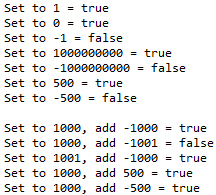
\includegraphics[scale=0.4]{test-illustrationer1.jpg}
\caption[<Text for the list of figures>]{Resultatet af testkørsel}
\label{fig:figure 2} 
\end{figure}
Dvs. hvis kontoen sættes til 1, bliver transaktionen gennemført (metoden returnerer ”true”). Hvis kontoen sættes til 0, bliver transaktionen ligeledes gennemført osv.
\\

Det interessante her er især grænseværdierne, dvs. netop 1, 0 og -1. Testen viser, at klassen opfører sig som vi ville forvente – en positiv værdi giver selvfølgelig true, men mere interessant, 0 giver også true. Ligeledes som forventet, returneres false, hvis balancen sættes til -1.
\\

Når grænseværdierne virker som forventet, vil alle værdier typisk gøre det, men for en sikkerheds skyld testes også lige med nogle meget store værdier, og med nogle helt almindelige værdier. Disse test giver også det forventede resultat.
\\

Herefter udføres en test hvor balancen først sættes til noget kendt, og derefter opdateres med ”addToAccount”. Ved den første test sættes balancen til 1000, hvorefter tilføjes -1000 – således må det forventes at den resulterende balance bliver 0. Dermed vil vi forvente at tranaktionen bliver fuldført, idet 0 ikke er negativt, og dermed er en godkendt værdi. Vi ser, at også denne test giver det forventede resultat.
\\

Sæt til 1000 og tilføj -1001 må give -1, og dermed false – OK.
Sæt til 1001 og tilføj -1000 må give 1, og dermed true – OK.
\\

De mere almindelige værdier giver ligeledes det forventede resultat. Således må det være fair at sige, at det er sandsynligt at en transaktion kun bliver gennemført, hvis ikke den resulterer i en negativ balance.
\\

\subsection{Test og fejlfinding generelt}
Foruden klassen til blackbox-test af Account-klassen, er der udviklet to test-klasser, som kan bruges til fejlfinding og test i programmet. Tanken er, at en eller begge test-klasser kan erstatte de ”rigtige” klasser, og på den måde give en udvikler mulighed for at teste scenarier, som er svære og/eller tidskrævende at opnå ved almindeligt spil.
\\

Der er dels tale om en GameBoard test-klasse, hvor værdierne for felterne alle er negative, således at sikringen af Account-klassen hurtigt kan testes i praksis. Derudover er der tale om en DieCup test-klasse, hvor en udvikler selv har mulighed for at sætte en fast værdi for hvad terningerne skal slå. Således kan der opnås at lande på f.eks. felt nr. 3 (som giver -200) mange gange i træk, og derved teste sikringen af Account-klassen, eller der kan landes på felt 12 (som giver +650) flere gange i træk, og derved teste de handlinger som udføres når en spiller vinder
\section{GRASP (General Responsibilty Assignment Software Patterns)}
Vi vil i dette afsnit beskrive de forskellige GRASP patterns og give eksempler på, hvordan vi har brugt det til implementering af vores program.
Connection between GRASP and UML page 277
\subsection{Controller}
Beskrivelse af en Controller
\subsubsection{Problem}
Hvilket objet under UI laget kontrollerer system operationer
\subsubsection{System operationer}
System operationer støder vi første gang på under analysen af \textbf{SSD} \textit{(System Sekvens Diagram)}. Dette er de vigtige hændelser i vores system.
For eksempel, når en spiller i vores spil trykker enter for at rulle med terningerne. Her starter han en system hændelse, der giver et terningeslag.
\\
En \textbf{Controller} er det første object under vores \textbf{UI} \textit{User Interface}, der har ansvar for at modtage eller løse system operations beskeder.
\subsubsection{Generel Løsning}
Tildel ansvaret til en klasse, som benytter en af følgende to valgmuligheder.
\begin{enumerate}
\item Klassen repræsenterer hovedsystemet med en slags "rod object". En enhed, sofwaren kører inden i systemet, eller et decideret subsystem - Dette er variationer af en \textit{Facade Controller}.
\item Klassen repræsenterer et use case scenarie hvor denne system handling ofte fremkommer. Denne vil tit være kaldet <UseCaseName>Handler, <UseCaseName>Coordinator eller <UseCaseName>Session.
\end{enumerate}
\subsubsection{Vores Løsning}
Vi har lavet en \textbf{Controller} kaldet \textit{GameController} til at styre vores sekvenser i spillet efter princippet med en \textit{Facade Controller}. 
\\
Det giver meget god mening at have en klasse, der uddelegerer ansvar. Dette gør at \textit{GameController} kun skal kontrollere og kordinere opgaver til andre objekter. Samtidig skal \textit{GameController} ikke udføre meget arbejde selv. Dette opfylder den guideline, der findes i \textit{Larman}
\subsection{Creater}
Beskrivelse af en Creator
\subsubsection{Problem}
Oprettelse af objekter, er en af de mest almindelige aktiviteter i et objektorienteret system.
\\
Et generelt princip til oprettelses ansvar er meget brugbart. Hvis ansvarsfordelingen bliver fordelt godt, kan man opnå \textbf{lav kobling} \textit{(Andet GRAS Pattern, der beskrives senere)}, større klarhed, indkapsling (den internne representation af et objekt, der er gemt fra kig udenfor objektets definition.) og genanvendelighed.
\subsubsection{Generel Løsning}
Giv klasse B ansvar for at oprette en instans af klassen A, hvis et af disse udtryk er sande (Helst flere af udtrykkenne).
\begin{itemize}
\item B indeholder, eller komposit agrigerer A
\item B bruger A tæt.
\item Bhar de initialiserende data til A, som bliver sendt til A, når denne er oprettet.
\\
Dermed er B \textbf{Expert} \textit{(Andet GRAS Pattern, der beskrives senere)} for at oprette A.
\end{itemize}
\subsubsection{Vores Løsning}
Denne tankegang har vi brugt i forbindelse med vores domænemodel. I den kan vi udlede at vores \textit{Game} bruger et \textit{GameBoard}, som indeholder flere \textit{Fields}. Vi kan dermed se at \textit{Game} er en god kandidat til at bære ansvaret for at oprette \textit{GameBoard}. \textit{GameBoard} er også oplagt til at oprette \textit{Field} objekter. Samme historie gentages i resten af modellen, så godt som muligt efter denne tankegang.
\subsection{Expert}
Beskrivelse af en Expert
\subsubsection{Problem}
Hvad er den gennerelle fremgangsmåde for at tildele ansvar til objekter.
\subsubsection{Generel Løsning}
Tildel ansvar til informations eksperten. Dette er klassen, der har de nødvendige informationer til at fuldfylde det ansvar.
\subsubsection{Vores Løsning}
Hvis vi kigger på eksempelvis vores \textit{DieCup}, har den ansvaret for at kende \textit{Die} terningeslag. Dermed er \textit{Diecup} expert i at få terningeslag.
\subsection{High Cohesion (Høj binding)}
Beskrivelse af High Cohesion
\subsubsection{Problem}
Hvordan holder man objekter fokuserede, forståelige og håndterbare og som en sideeffekt benytter lav kobling \textit{(Andet GRAS Pattern, der beskrives senere)}
\subsubsection{Generel Løsning}
Tildel ansvar, så bindingen forbliver høj. Brug dette til at vurdere alternativer.
\\
En klasse med lav binding laver mange urelaterede ting, eller har for mange opgaver.
\\
Sådanne klasser ønskes ikke fordi de kan være:
\begin{itemize}
\item Svær at forstå
\item Svær at genanvende
\item Konstant udsat for forandringer
\end{itemize}
Klasser med lav binding har tit for meget ansvar, som kunne uddelegeres til andre objekter.
\subsubsection{Vores Løsning}
Et godt eksempel i vores program, er at vores \textit{Game}klasse,  holder styr på spillerne i \textit{Player} klassen. Istedet for at \textit{Game} også holder styr på spillerens pengebeholdning, har vi givet ansvaret til \textit{Player}, som holder styr på \textit{Account}.
\subsection{Indirection}
Beskrivelse af Indirection
\subsubsection{Problem}
Hvor skal man tildele et ansvarsområder, for at undgå direkte kobling mellem to eller flere ting?
\\
Hvordan afkobler man objekter, så man opnår lav kobling, og genanvendelsesmuligheder forbliver høje.
\subsubsection{Generel Løsning}
Giv ansvaret til et mellemliggende objekt til at kommunikere mellem andre komponenter, så de ikke er direkte sammenkoblet.
\\
Det mellemliggende objekt laver en \textit{inderection} mellem de andre komponenter.
\subsubsection{Vores Løsning}
Vi har forsøgt at bruge \textit{Inderection}, ved at lave en \textit{Graphic} klasse, der holder styr på alt, der foregår i forhold til at kalde vores eksterne GUI. Dette gjorde vi for, at det ville være nemmere at lave spillet om, hvis der skulle ske modifikationer i GUI biblioteket. Dette skete rent faktisk, da vi var midt i projektet. Vi fik besked om at GUI'en, nu var blevet ændret. Selvom vi syntes det var lidt irriterende, kunne vi hurtigt rette det til, da vi kun skulle rette i den ene klasse.
\subsection{Low Coupling (Lav kobling)}
Beskrivelse af Low Coupling
\subsubsection{Problem}
Hvordan opnår man lav afhængighed. lav forandrings indvirkning og forhøjet genanvendelse.
\\
\textbf{Coubling} er et mål for hvor stærkt et element er koblet til, har kendskab til eller er afhængig af andre elementer.
\\
En klasse med høj kobling afhænger af mange klasser. Sådanne klasser kan være uønskede. De kan lide af følgende problemer.
\begin{itemize}
\item Tvunge lokale forandringer på grund af forandringer i sammenhængende klasser.
\item Sværere at forstå i isolerede tilfælde.
\item Sværere at genanvende, da det vil kræve tilhørende tilstedeværelse af afhængige klasser.
\end{itemize}
\subsubsection{Generel Løsning}
Tildel ansvar, så koblingen forbliver lav. Brug dette princip til at evaluere alternativer.
\subsubsection{Vores Løsning}
Dette er forsøgt implementeret i for eksempel vores \textit{Game}, der istedet for at kalde til  \textit{Player} for bagefter at kalde \textit{Account}, og dermed skabe høj kobling, har vi valgt at kalde \textit{Account} igennem \textit{Player} klassen. Dette sikrer en lav kobling, men samtidig også høj binding, da man sjældent kan bruge principperne alene.
\subsection{Polymorphism}
Beskrivelse af Polymorphism
\subsubsection{Problem}
Hvordan opretter man alternativer baseret på typer eller software, der kan kobles direkte på de allerede eksisterende komponenter.
\textit{Alternativer baseret på typer} - Hvis et program er designet med et if-else eller switch statement, og en ny variation opstår, kan det ofte betyde ændringer mange steder i koden. Denne fremgangsmåde gør det besværligt at udvide et program på en nem måde. Dette er fordi, ændringerne skal foretages flere forskellige steder, hvor denne betingelses logik er implementeret.
\subsubsection{Generel Løsning}
Når familiære alternativer eller opførsel varierer efter type (klasse), gives ansvaret for opførslen til typerne, hvori opførslen varierer. Dette gøres ved at bruge polymorfiske operatgioner.
\subsubsection{Vores Løsning}
Vi har ikke benyttet polymorphi i vores spil. Vi har dog tænkt på, at vores felter måske i fremtiden, vil komme til at være af forskellige typer. Dermed kan det blive aktuelt at benytte mønstret for polymorfi ved en eventuel opdatering af spillet.
\subsection{Protected Variations}
Beskrivelse af Protected Variations
\subsubsection{Problem}
Hvordan tildeler man ansvar til objekter, subsystemer eller systemer, så variationer og ustabilitet i disse elementer ikke får en uønsket effekt på andre elementer.
\subsubsection{Generel Løsning}
Identificer punkter med uønsket variation eller ustabilitet. Lav en stabil grænseflade om dem. Dette bruges tit i forbindelse med polymorfi.
\subsubsection{Vores Løsning}
I vores spil har det ikke været nødvendigt at bruge dette mønster.
\subsection{Pure Fabrication}
Beskrivelse af Pure Fabrication
\subsubsection{Problem}
Objekt orienterede designs er nogle gange karakteriserede ved at tage udgangspunkt i problemdomæner fra den virkelige verden, for at lette forståelsen. For eksempel \textit{Gameboard} og \textit{Field} klasserne. Nogle gange kan der der opstå situationer, hvor det giver problemer kun at tildele ansvar til domæne lags klasser. Det kan give dårlig binding, kobling eller lav genanvedelsesmulighed.
\subsubsection{Generel Løsning}
Giv et sæt ansvarsopgaver med høj sammenhæng til en kunstig eller belejelig klasse, der ikke er repræsenteret i domænelaget. Denne opfundne klasse skal supportere høj binding, lav kobling og være nem at genbruge.
\subsubsection{Vores Løsning}
Vi har opfundet klasser til at håndtere det grafiske i spillet med klassen \textit{Graphic}, og den tekstbaserede del kørers i klassen \textit{TUI}. Disse klasser opfylder ovenstående krav.
\section{Design sekvens-diagram}
\todo[inline]{Chris: tegn diagram og forklar}
\begin{figure}[!ht]
\centering
\includegraphics[width=1\textwidth]{DSD.pdf}
\caption[<Text for the list of figures>]{Design Sekvens Diagram}
\label{fig:figure2}
\end{figure}
\newpage
Vi har, som ved første spil,  lavet et design sekvens-diagram, som dokumenterer, hvordan koden bliver udført sekventielt, når man spiller det nye feltspil. Hvis man sammenligner vores sekvensdiagram med vores kode afsnit, vil man se at \textit{Game} controlleren har det primære ansvar for at fordele opgaverne rundt til de ande dele af programmet. Her kan vi bare se det ud fra et tidsmæssigt perspektiv istedet. Hvordan de forskellige metodekald virker, kan man nærstudere i vores afsnit om selve koden.
\\

Desværre er diagrammet fyldt med forkert syntaks og variabler, der er brugt som metodekald. Da dette er noget af det sidste vi har lavet i vores dokumentation, har tidsgrænsen bevirket, vi ikke har kunnet afhjælpe disse fejl inden for den ønskede tidsramme.
\\
Vi vil dog anbefale, at man får dette rettet hurtigst muligt, hvis der er planer om eventuelle opdateringer til spillet, eller genbrug af dele af systemet.
\section{Design-klassediagram}
Her kan man se vores Design Klasse Diagram. Hvis man kigger nok på det, vil man se at der er masser af pile, men ingen af dem har nogen der går retur. Det vil sige det er lykkedes os på en nogenlundef ornuftig måde at overholde de fleste patterns i \textbf{GRASP}.
Dette ses i figur \vref{fig:design}.
\begin{figure}[!ht]
\centering
\includegraphics[width=1\textwidth]{ClassDiagram.pdf}
\caption[<Text for the list of figures>]{Design-Klassediagram}
\label{fig:design}
\end{figure}
\newpage
\section{Kildeliste}
Her vil vi oplyse om hvilke kilder, der er brugt til rapporten.
Vi vil både oplyse om hvilke bøger, hjemmesider og software vi har brugt.
\printbibliography %Print the bibliography set under \bibliography.
\section{Anvendte værktøjer}
\begin{itemize}
\item \textbf{Eclipse - kepler}. Brugt som vores værktøj til at kode java i.
\item \textbf{UMLet}. Foretrukket værktøj til \textbf{UML} diagrammer.
\item \textbf{Dropbox}. Brugt til at dele filer imellem os. 
\item \textbf{TexMaker}. Brugt for at skabe en flot rapport skrevet i \LaTeX
\end{itemize}
\newpage
\section{Bilag}
\subsection{Kode}
Her vil hele vores kode til programmet være repræsenteret som bilag.
\subsubsection{TUI - Boundary}
\lstinputlisting[language = Java, tabsize = 2,stringstyle=\color{myblue},commentstyle=\color{mygreen},showstringspaces = false, breaklines=true, numbers = left,keywordstyle = \bfseries\color{mymauve}]{TUI.java}
\subsubsection{Graphic - Boundary}
\lstinputlisting[language = Java, tabsize = 2,stringstyle=\color{myblue},commentstyle=\color{mygreen},showstringspaces = false, breaklines=true, numbers = left,keywordstyle = \bfseries\color{mymauve}]{Graphic.java}
\subsubsection{Main - Controller}
\lstinputlisting[language = Java, tabsize = 2,stringstyle=\color{myblue},commentstyle=\color{mygreen},showstringspaces = false, breaklines=true ,numbers = left,keywordstyle = \bfseries\color{mymauve}]{Main.java}
\subsubsection{Game - Controller}
\lstinputlisting[language = Java, tabsize = 2,stringstyle=\color{myblue},commentstyle=\color{mygreen},showstringspaces = false, breaklines=true, numbers = left,keywordstyle = \bfseries\color{mymauve}]{Game.java}
\subsubsection{Player - Entity}
\lstinputlisting[language = Java, tabsize = 2,stringstyle=\color{myblue},commentstyle=\color{mygreen},showstringspaces = false, breaklines=true, numbers = left,keywordstyle = \bfseries\color{mymauve}]{Player.java}
\subsubsection{Account - Entity}
\lstinputlisting[language = Java, tabsize = 2,stringstyle=\color{myblue},commentstyle=\color{mygreen},showstringspaces = false,breaklines=true, numbers = left,keywordstyle = \bfseries\color{mymauve}]{Account.java}
\subsubsection{Gameboard - Entity}
\lstinputlisting[language = Java, tabsize = 2,stringstyle=\color{myblue},commentstyle=\color{mygreen},showstringspaces = false,breaklines=true, numbers = left,keywordstyle = \bfseries\color{mymauve}]{Gameboard.java}
\subsubsection{Field - Entity}
\lstinputlisting[language = Java, tabsize = 2,stringstyle=\color{myblue},commentstyle=\color{mygreen},showstringspaces = false,breaklines=true, numbers = left,keywordstyle = \bfseries\color{mymauve}]{Field.java}
\subsubsection{Ownable - Entity}
\lstinputlisting[language = Java, tabsize = 2,stringstyle=\color{myblue},commentstyle=\color{mygreen},showstringspaces = false,breaklines=true, numbers = left,keywordstyle = \bfseries\color{mymauve}]{Ownable.java}
\subsubsection{Fleet - Entity}
\lstinputlisting[language = Java, tabsize = 2,stringstyle=\color{myblue},commentstyle=\color{mygreen},showstringspaces = false,breaklines=true, numbers = left,keywordstyle = \bfseries\color{mymauve}]{Fleet.java}
\subsubsection{LaborCamp - Entity}
\lstinputlisting[language = Java, tabsize = 2,stringstyle=\color{myblue},commentstyle=\color{mygreen},showstringspaces = false,breaklines=true, numbers = left,keywordstyle = \bfseries\color{mymauve}]{LaborCamp.java}
\subsubsection{Refuge - Entity}
\lstinputlisting[language = Java, tabsize = 2,stringstyle=\color{myblue},commentstyle=\color{mygreen},showstringspaces = false,breaklines=true, numbers = left,keywordstyle = \bfseries\color{mymauve}]{Refuge.java}
\subsubsection{Tax - Entity}
\lstinputlisting[language = Java, tabsize = 2,stringstyle=\color{myblue},commentstyle=\color{mygreen},showstringspaces = false,breaklines=true, numbers = left,keywordstyle = \bfseries\color{mymauve}]{Tax.java}
\subsubsection{Territory - Entity}
\lstinputlisting[language = Java, tabsize = 2,stringstyle=\color{myblue},commentstyle=\color{mygreen},showstringspaces = false,breaklines=true, numbers = left,keywordstyle = \bfseries\color{mymauve}]{Territory.java}
\subsubsection{DieCup - Entity}
\lstinputlisting[language = Java, tabsize = 2,stringstyle=\color{myblue},commentstyle=\color{mygreen},showstringspaces = false, breaklines=true, numbers = left,keywordstyle = \bfseries\color{mymauve}]{DieCup.java}
\subsubsection{Die - Entity}
\lstinputlisting[language = Java, tabsize = 2,stringstyle=\color{myblue},commentstyle=\color{mygreen},showstringspaces = false,breaklines=true, numbers = left,keywordstyle = \bfseries\color{mymauve}]{Die.java}
\subsubsection{DieCupTestEntity - TestTools}
\lstinputlisting[language = Java, tabsize = 2,stringstyle=\color{myblue},commentstyle=\color{mygreen},showstringspaces = false, breaklines=true, numbers = left,keywordstyle = \bfseries\color{mymauve}]{DieCupTestEntity.java}
\subsubsection{FleetTest - TestTools}
\lstinputlisting[language = Java, tabsize = 2,stringstyle=\color{myblue},commentstyle=\color{mygreen},showstringspaces = false, breaklines=true, numbers = left,keywordstyle = \bfseries\color{mymauve}]{FleetTest.java}
\subsubsection{LaborCampTest - TestTools}
\lstinputlisting[language = Java, tabsize = 2,stringstyle=\color{myblue},commentstyle=\color{mygreen},showstringspaces = false, breaklines=true, numbers = left,keywordstyle = \bfseries\color{mymauve}]{LaborCampTest.java}
\subsubsection{RefugeTest - TestTools}
\lstinputlisting[language = Java, tabsize = 2,stringstyle=\color{myblue},commentstyle=\color{mygreen},showstringspaces = false, breaklines=true, numbers = left,keywordstyle = \bfseries\color{mymauve}]{RefugeTest.java}
\subsubsection{TaxTest - TestTools}
\lstinputlisting[language = Java, tabsize = 2,stringstyle=\color{myblue},commentstyle=\color{mygreen},showstringspaces = false, breaklines=true, numbers = left,keywordstyle = \bfseries\color{mymauve}]{TaxTest.java}
\subsubsection{TerritoryTest - TestTools}
\lstinputlisting[language = Java, tabsize = 2,stringstyle=\color{myblue},commentstyle=\color{mygreen},showstringspaces = false, breaklines=true, numbers = left,keywordstyle = \bfseries\color{mymauve}]{TerritoryTest.java}
\end{document}